\begin{subfigure}{0.3\textwidth}
\centering
\fbox{\begin{tikzpicture}
\draw[fill] (0,0) circle (2pt) coordinate (a);
\draw[fill] (0.4,3) circle (2pt) coordinate (b);
\draw[fill] (2,3.4) circle (2pt) coordinate (c);
\draw[fill] (3.5,0.7) circle (2pt) coordinate (d);
\draw[fill] (1,1) circle (2pt) coordinate (e);
\draw[fill] (2,2) circle (2pt) coordinate (f);
\draw[fill] (3,0.7) circle (2pt) coordinate (g);
\end{tikzpicture}}
\caption{Initial configuration.}
\label{subfig:increasing_loop_step_0}
\end{subfigure}
\begin{subfigure}{0.3\textwidth}
\centering
\fbox{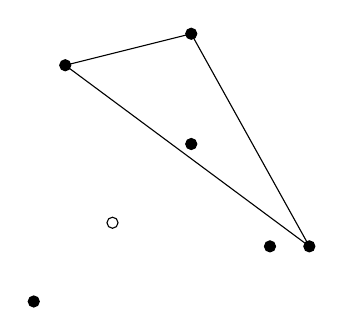
\begin{tikzpicture}
\draw[fill] (0,0) circle (2pt) coordinate (a);
\draw[fill] (0.4,3) circle (2pt) coordinate (b);
\draw[fill] (2,3.4) circle (2pt) coordinate (c);
\draw[fill] (3.5,0.7) circle (2pt) coordinate (d);
\draw[] (1,1) circle (2pt) coordinate (e);
\draw[fill] (2,2) circle (2pt) coordinate (f);
\draw[fill] (3,0.7) circle (2pt) coordinate (g);
\draw (b)--(d);
\draw (b)--(c);
\draw (c)--(d);
\end{tikzpicture}}
\caption{Initialisation.}
\label{subfig:increasing_loop_step_1}
\end{subfigure}
\begin{subfigure}{0.3\textwidth}
\centering
\fbox{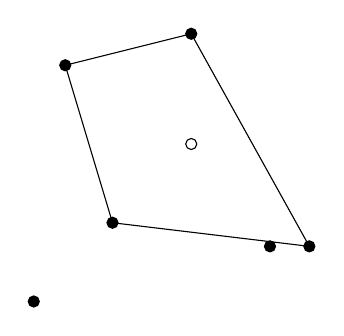
\begin{tikzpicture}
\draw[fill] (0,0) circle (2pt) coordinate (a);
\draw[fill] (0.4,3) circle (2pt) coordinate (b);
\draw[fill] (2,3.4) circle (2pt) coordinate (c);
\draw[fill] (3.5,0.7) circle (2pt) coordinate (d);
\draw[fill] (1,1) circle (2pt) coordinate (e);
\draw[] (2,2) circle (2pt) coordinate (f);
\draw[fill] (3,0.7) circle (2pt) coordinate (g);
\draw (b)--(e);
\draw (e)--(d);
\draw (b)--(c);
\draw (c)--(d);
\end{tikzpicture}}
\caption{First addition.}
\label{subfig:increasing_loop_step_2}
\end{subfigure}
\vspace{1ex}\\
\begin{subfigure}{0.3\textwidth}
\centering
\fbox{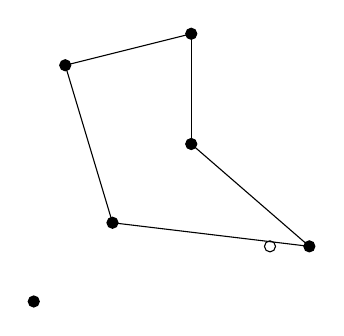
\begin{tikzpicture}
\draw[fill] (0,0) circle (2pt) coordinate (a);
\draw[fill] (0.4,3) circle (2pt) coordinate (b);
\draw[fill] (2,3.4) circle (2pt) coordinate (c);
\draw[fill] (3.5,0.7) circle (2pt) coordinate (d);
\draw[fill] (1,1) circle (2pt) coordinate (e);
\draw[fill] (2,2) circle (2pt) coordinate (f);
\draw[] (3,0.7) circle (2pt) coordinate (g);
\draw (b)--(e);
\draw (e)--(d);
\draw (b)--(c);
\draw (c)--(f);
\draw (f)--(d);
\end{tikzpicture}}
\caption{Intermediate addition.}
\label{subfig:increasing_loop_step_3}
\end{subfigure}
\begin{subfigure}{0.3\textwidth}
\centering
\fbox{\begin{tikzpicture}
\draw[] (0,0) circle (2pt) coordinate (a);
\draw[fill] (0.4,3) circle (2pt) coordinate (b);
\draw[fill] (2,3.4) circle (2pt) coordinate (c);
\draw[fill] (3.5,0.7) circle (2pt) coordinate (d);
\draw[fill] (1,1) circle (2pt) coordinate (e);
\draw[fill] (2,2) circle (2pt) coordinate (f);
\draw[fill] (3,0.7) circle (2pt) coordinate (g);
\draw (b)--(e);
\draw (b)--(c);
\draw (c)--(f);
\draw (f)--(d);
\draw (g)--(d);
\draw (g)--(e);
\end{tikzpicture}}
\caption{Final addition.}
\label{subfig:increasing_loop_step_4}
\end{subfigure}
\begin{subfigure}{0.3\textwidth}
\centering
\fbox{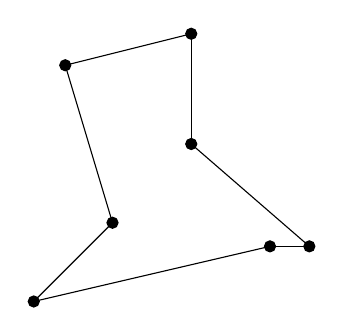
\begin{tikzpicture}
\draw[fill] (0,0) circle (2pt) coordinate (a);
\draw[fill] (0.4,3) circle (2pt) coordinate (b);
\draw[fill] (2,3.4) circle (2pt) coordinate (c);
\draw[fill] (3.5,0.7) circle (2pt) coordinate (d);
\draw[fill] (1,1) circle (2pt) coordinate (e);
\draw[fill] (2,2) circle (2pt) coordinate (f);
\draw[fill] (3,0.7) circle (2pt) coordinate (g);
\draw (b)--(e);
\draw (b)--(c);
\draw (c)--(f);
\draw (f)--(d);
\draw (g)--(d);
\draw (g)--(a);
\draw (e)--(a);
\end{tikzpicture}}
\caption{Final route.}
\label{subfig:increasing_loop_step_5}
\end{subfigure}